\documentclass[onecolumn, oneside, a4paper, 11pt]{memoir}

\usepackage[utf8]{inputenc}
\usepackage[T1]{fontenc}

% Paths
\newcommand{\figs}{../figs}
\newcommand{\data}{../data}

% Fonts
\usepackage{newpxtext,newpxmath}
\renewcommand*\sfdefault{cmss}

% References
\usepackage{hyperref}

% Units
\usepackage[detect-weight=true, binary-units=true]{siunitx}
\DeclareSIUnit\flop{Flops}

% Math
\let\openbox\undefined
\usepackage{amsthm}
\usepackage{amsmath}
\usepackage{amssymb}
\usepackage{bm}

\theoremstyle{remark}
\newtheorem{ex}{Exercise}
\newtheorem*{sol}{Solution}

% Graphics
\usepackage{graphicx}
\usepackage{caption}
\usepackage{subcaption}
\graphicspath{{../figs/}}

% Tikz
\usepackage{tikz}
\usetikzlibrary{positioning,shapes,arrows,calc,intersections}
\usepackage{pgfplots}
\usepgfplotslibrary{dateplot}
\pgfplotsset{compat=1.8}

% Colors
\definecolor{darkblue}{HTML}{00688B}
\definecolor{darkgreen}{HTML}{6E8B3D}
\definecolor{cadet}{HTML}{DAE1FF}
\definecolor{salmon}{HTML}{FFB08A}

% Listings
\usepackage{textcomp}
\usepackage{listings}
\lstset{
  keywordstyle=\bfseries\color{orange},
  stringstyle=\color{darkblue!80},
  commentstyle=\color{darkblue!80},
  showstringspaces=false,
  basicstyle=\ttfamily,
  upquote=true,
}
\lstdefinestyle{fortran}{
  language=Fortran,
  morekeywords={for},
  deletekeywords={status},
}
\lstdefinestyle{c}{
  language=C,
  morekeywords={include},
}
\lstdefinestyle{shell}{
  language=bash,
}

\begin{document}

\pagestyle{empty}

\begin{center}
  {\Huge \bfseries \scshape
    Introduction to \\[0.2\baselineskip] Supercomputing} \\[2\baselineskip]
  {\Large TMA4280 $\cdot$ Problem set 2} \\[2\baselineskip]
\end{center}

\begin{ex}
  The previous supercomputer at NTNU, \emph{Njord}, was based on the POWER5
  dual-core chip, which had cache sizes:
  \begin{itemize}
  \item L1: $\SI{32}{\kilo\byte}$,
  \item L2: $\SI{1.875}{\mega\byte}$,
  \item L3: $\SI{36}{\mega\byte}$.
  \end{itemize}
  Assuming double precision, how many floating point numbers can fit in each
  cache? What is the dimension of the largest square matrix that can fit in each
  cache?
\end{ex}

\begin{ex}
  What limits are there to the speed of electronic circuits?

  What is the maximum distance a memory unit could be from an arithmetic unit
  (in a processor), and still allow a memory access time of
  $\SI{100}{\pico\second}$? ($\SI{1}{\pico\second} = 10^{-12}\,\SI{}{\second}$.)
\end{ex}

\begin{ex}
  Assume that we have a scalar $c$ and two vectors $\bm a$ and $\bm b$ of length
  $n$. We consider three types of linear algebra operations:
  \begin{itemize}
  \item Add $c$ to all elements in $\bm a$.
  \item Add $\bm a$ and $\bm b$ and store the result in $\bm a$.
  \item Multiply $\bm b$ with $c$ and add $\bm a$ to the resulting vector. Store
    the result in $\bm a$.
  \end{itemize}

  Below we show three Fortran subroutines implementing these operations,
  however, the particular choice of programming language doesn't matter.
  \begin{lstlisting}[style=fortran]
subroutine op1(a,c,n)
  real a(n),c
  do i=1,n
    a(i) = a(i) + c
  end do
  return
end
  \end{lstlisting}
  \begin{lstlisting}[style=fortran]
subroutine op2(a,b,n)
  real a(n),b(n)
  do i=1,n
    a(i) = a(i) + b(i)
  end do
  return
end
  \end{lstlisting}
  \begin{lstlisting}[style=fortran]
subroutine op3(a,b,n)
  real a(n),b(n),c
  do i=1,n
    a(i) = a(i) + c*b(i)
  end do
  return
end
  \end{lstlisting}

  These three routines were tested on an older supercomputer at NTNU around the
  year 2000. In order to check the single-processor performance, a test program
  was run which called each of these routines many times. The mean number of
  floating-point operations for different vector lengths $n$ was then computed.
  The results are summarized in the following figure.

  \begin{figure}[htbp]
    \begin{center}
      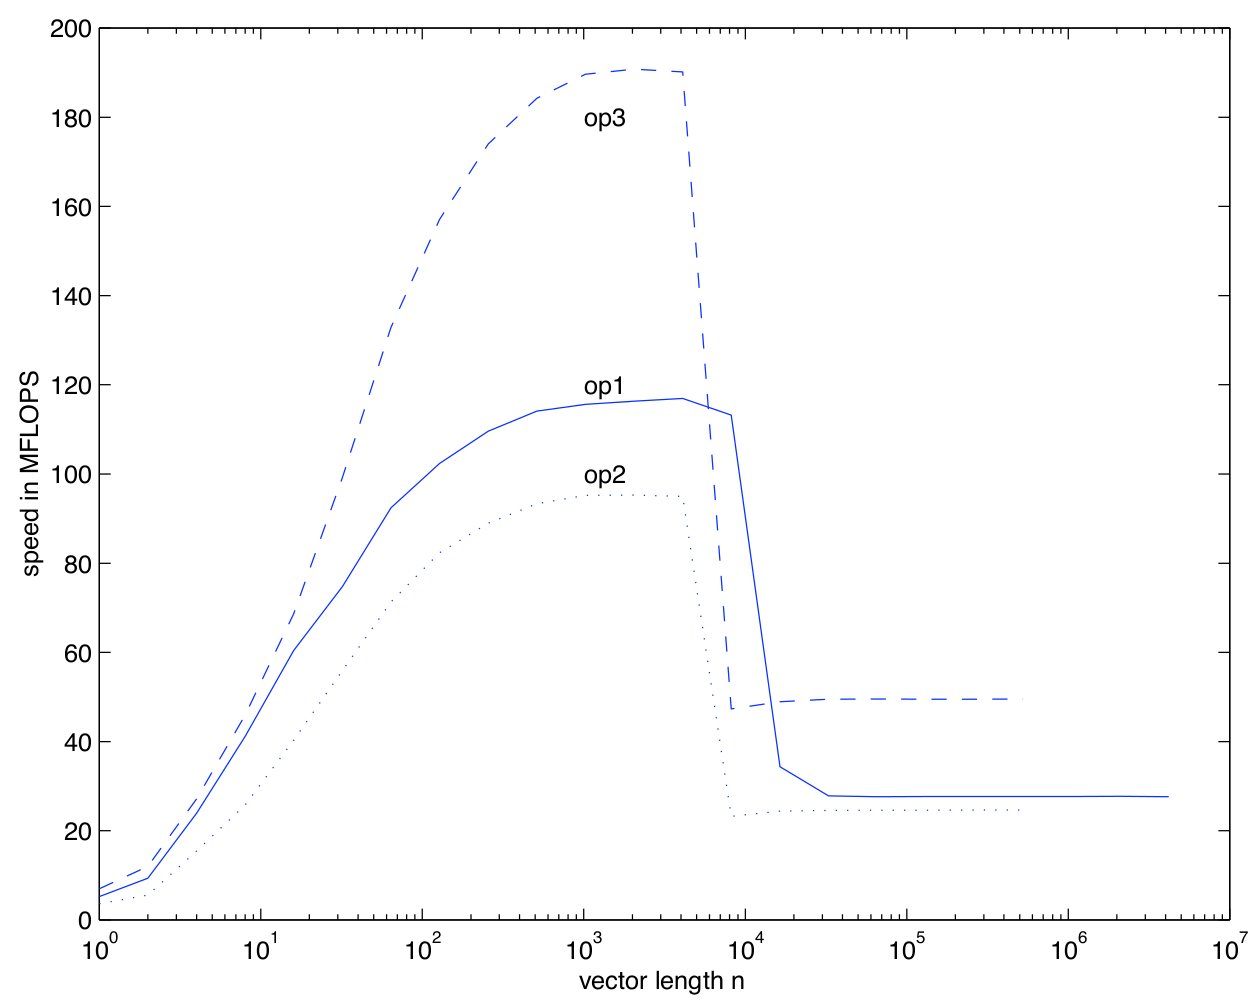
\includegraphics[width=0.5\textwidth]{ctest}
    \end{center}
    \caption{Performance on a single alpha chip on a Cray T3E supercomputer.}
  \end{figure}

  Explain these results. In particular,
  \begin{itemize}
  \item Why does the speed increase with $n$ for small $n$, followed by being
    largely independent of $n$?
  \item Why is there a sudden drop at a particular vector length?
  \item Why does this drop happen sooner for operations 2 and 3 than for
    operation 1? (At $n=4096$ and $n=8192$ respectively. This is difficult to
    see in the figure.)
  \item Why does operation 1 run faster than operation 3, and why does operation
    2 run slower still?
  \end{itemize}
\end{ex}

\begin{ex}
  Consider the vector operation $\bm c = \bm a + \bm b$, where all vectors are
  of length $n$. One way to implement this operation is:
  \begin{lstlisting}[style=fortran]
for i=1,n
  c(i) = a(i) + b(i)
end
  \end{lstlisting}
  To maximize perfomance, we want to ensure that the vector elements are stored
  interleaved in memory:
  \[
    \ldots, a_i, b_i, c_i, a_{i+1}, b_{i+1}, c_{i+1}, \ldots
  \]
  \begin{itemize}
  \item Why could this storage scheme be advantageous?
  \item How would you realize this in C and/or in Fortran?
  \item Do you think this scheme would pay off compared to the extra
    implementation effort?
  \end{itemize}
\end{ex}

\begin{ex}
  Implement a program in C or Fortran which performs the following three
  different operations:
  \begin{align*}
    \bm x &= \bm a + \gamma \bm b \\
    \bm y &= \bm a + \bm A \bm b \\
    \alpha &= \bm x^\intercal \bm y
  \end{align*}
  You can use any compatible vectors and matrices you see fit (e.g. random
  ones). The constant $\gamma$ should be read from the command line.
\end{ex}

\end{document}
